\subsection{ResNet50}\label{s:resnet50}
\chapterauthor{Benjamin Loh Choon How (2201590)}

ResNet50 \cite{He_Zhang_Ren_Sun_2015} is a transformative convolutional neural network (CNN) architecture developed by Microsoft Research that introduces residual learning to address the challenges of training deep networks. By using residual connections, or "skip connections," the model facilitates the direct propagation of gradients across layers, effectively mitigating the vanishing gradient problem. This allows ResNet50 to maintain performance and stability even as the network depth increases, enabling the extraction of complex features from input data. The architecture consists of multiple stages, starting with initial pre-processing layers like zero-padding, convolution, batch normalization, ReLU activation, and max pooling, which prepare the data for deeper processing. These are followed by several residual blocks across different stages, each comprising a sequence of convolutional layers interspersed with identity blocks that implement the skip connections, preserving the flow of information and enhancing learning efficiency.

\begin{figure}[H]
  \begin{center}
    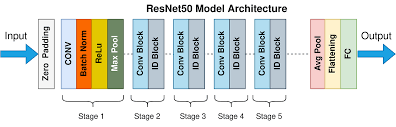
\includegraphics[width=0.7\textwidth]{resnet50/resnet50_architecture.png}
  \end{center}
  \caption{Resnet50 Architecture}\label{f:resnet50_architecture}
\end{figure}

The final stages of ResNet50 involve a global average pooling layer that reduces feature maps to a single vector per map, significantly lowering the number of parameters and computational complexity. This is followed by a fully connected layer that outputs class probabilities, making the model suitable for classification tasks. The design of ResNet50, as seen in Figure \ref{f:resnet50_architecture}, showcases its capability to transform high-dimensional data into compact, meaningful representations. This robust architecture has been widely adopted for various applications, excelling in tasks such as image classification and object detection, making it a cornerstone in deep learning for handling complex visual analysis with high accuracy and efficiency.

\subsubsection{Implementation}

For our brain tumor classification task, we utilized the ResNet50 model pretrained on the ImageNet dataset. This pre-training provides a robust feature extraction base, which we then tailored to our specific task through further training and adaptation. The ResNet50 architecture begins with the standard base model loaded with ImageNet weights but excludes the top layers to better suit our specialized classification needs. The input shape is set to $224\times224$ with three channels, ensuring the input images are resized to match these dimensions during preprocessing. This alignment enhances the classification accuracy by fitting the images into the network's expected input format.

Following the base layers, we introduced a Global Average Pooling 2D layer. This layer reduces the spatial dimensions of the feature maps to a single vector per map, effectively summarizing the most critical features while significantly minimizing the number of parameters and the computational burden. This pooling step is crucial for maintaining efficiency and avoiding overfitting. Next, a Dropout layer with a 40\% drop rate is included, which randomly disables a fraction of the neurons during training. This randomness helps prevent overfitting by ensuring the model does not rely too heavily on any specific set of neurons, promoting the development of redundant pathways that sustain performance even if some neurons are inactive.

The network culminates in a Dense layer with four units, each corresponding to one of the brain tumor classes: meningioma, glioma, pituitary, and notumor. This layer employs a softmax activation function to output the probability distribution over the tumor classes, providing a clear, interpretable classification result. The model was compiled using the Adam optimizer with a starting learning rate of $0.0001$ and a categorical cross-entropy loss function, which is appropriate for this multi-class classification scenario. This combination offers a balance between rapid convergence and precise adjustments during training, optimizing the model's performance metrics, including accuracy.

Training was conducted over 80 epochs with a series of callbacks to optimize performance and prevent overfitting. These included \textit{ModelCheckpoint} to save the best version of the model based on validation loss and \textit{EarlyStopping} to halt training when no improvement in validation loss was observed for a specified number of epochs, preventing unnecessary overtraining. The training process was halted early at epoch 50, with a batch size of 10. The model was trained on the training set and validated on the validation set, with the best validation accuracy model saved as the final model. Upon evaluation on the test set, the model achieved an accuracy of 0.9973 and a validation accuracy of 0.9111, with a validation loss of 0.2656. These performance metrics are detailed in Table \ref{tab:resnet50_classification_report} and Table \ref{tab:resnet50_additional_metrics}, reflecting the model's robust and reliable performance.

\subsubsection{Fine-Tuning}

In the fine-tuning phase of the ResNet50 model, the Optuna package was employed to systematically explore and optimize the hyperparameters, particularly focusing on the dropout rate. The goal of this process was to identify the most effective dropout rate that balances model performance and overfitting with the least validation loss. Through multiple trials, each testing a different dropout rate within the range of 0.1 to 0.5, the optimal dropout rate was found to be the original at 0.4, which provided a balance between mitigating overfitting and maintaining model performance. This specific dropout rate was thus adopted in the final model architecture.

The overall approach demonstrates the rigorous method employed to fine-tune the model, ensuring optimal performance for brain tumor segmentation. By leveraging advanced optimization techniques and thoroughly validating the model, this work contributes to the development of more accurate and reliable medical imaging models.

Table \ref{tab:finetuning_results} summarizes the results of the fine-tuning trials, listing the validation loss for each tested dropout rate.

\begin{longtable}{|c|c|}
\caption{Fine-Tuning Results for Different dropout rates}\label{tab:finetuning_results}
\hline
\textbf{Dropout Rate} & \textbf{Validation Loss}
\hline
\endfirsthead
\hline
\textbf{Dropout Rate} & \textbf{Validation Loss}
\hline
\endhead
\hline
\endfoot
\hline
\endlastfoot
0.3480 (Trial 1) & 0.3926
\hline
0.1964 (Trial 2) & 0.4379
\hline
0.3836 (Trial 3) & 0.4648
\hline
0.2228 (Trial 4) & 0.2663
\hline
0.3506 (Trial 5) & 0.4114
\end{longtable}

The Optuna optimization process involved defining a model creation function that took a dropout rate as a parameter, suggested by Optuna for each trial. For each trial, a ResNet50-based model was constructed with varying dropout rates and trained for 35 epochs using the Adam optimizer. The training process included callbacks for early stopping based on validation loss. The minimum validation loss achieved during each trial served as the objective metric for evaluating the performance of the model.

During the fine-tuning trials, different dropout rates were tested to optimize the model's performance. Among the configurations, a dropout rate of 0.2228 achieved the lowest validation loss of 0.2663, significantly outperforming other rates. Although a dropout rate of 0.3480 showed promising results with a validation loss of 0.3926 in Trial 1, the dropout rate of 0.2228 was observed to provide a better balance, yielding the lowest validation loss across the trials. Despite these, the original dropout rate of 0.4 seems to have the best performance with a validation loss of 0.2656 therefore it will be used as the final model for evaluation.

The fine-tuning process underscored the significance of dropout rate selection in enhancing the model's performance and contributing to the model's effectiveness in accurately segmenting brain tumors. The results are summarized in Table \ref{tab:finetuning_results}.

\subsubsection{Results and Evaluation}

\begin{figure}[H]
  \centering
  \begin{subfigure}[b]{0.2\textwidth}
    \centering
    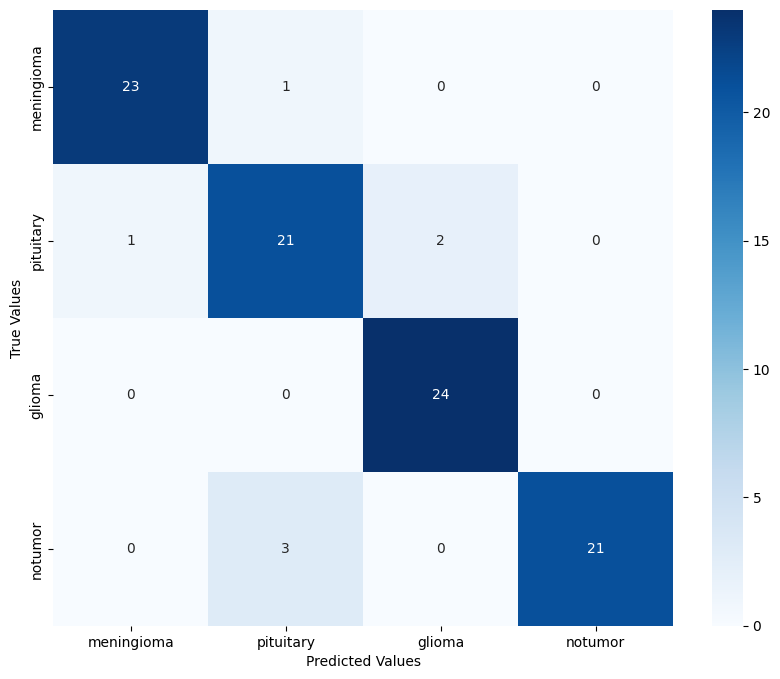
\includegraphics[width=\textwidth]{resnet50/evaluation/cm1.png}
    \caption{Confusion Matrix}
    \label{fig:resnet50_cm1}
  \end{subfigure}
  \hfill
  \begin{subfigure}[b]{0.2\textwidth}
    \centering
    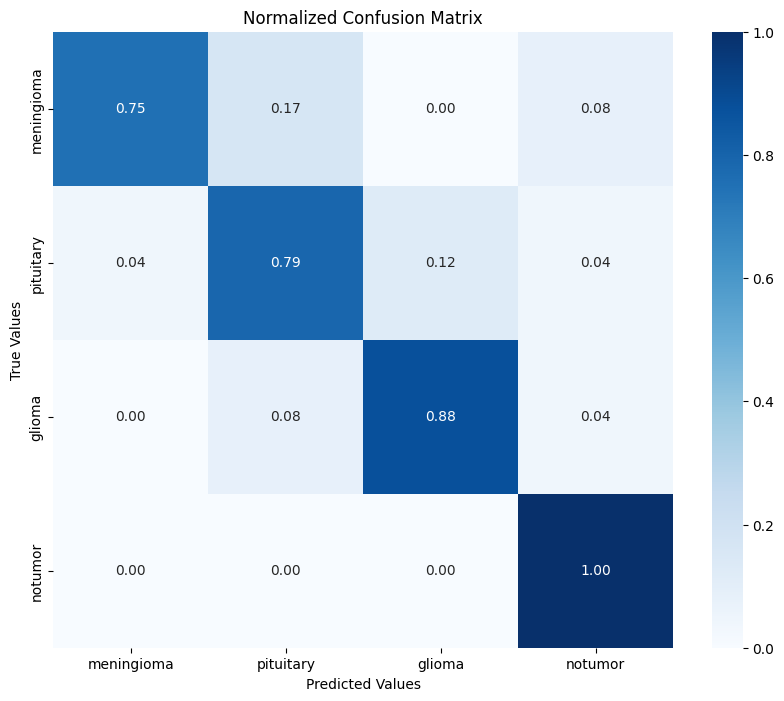
\includegraphics[width=\textwidth]{resnet50/evaluation/cm2.png}
    \caption{Normalized Confusion Matrix}
    \label{fig:resnet50_cm2}
  \end{subfigure}
  \hfill
  \begin{subfigure}[b]{0.25\textwidth}
    \centering
    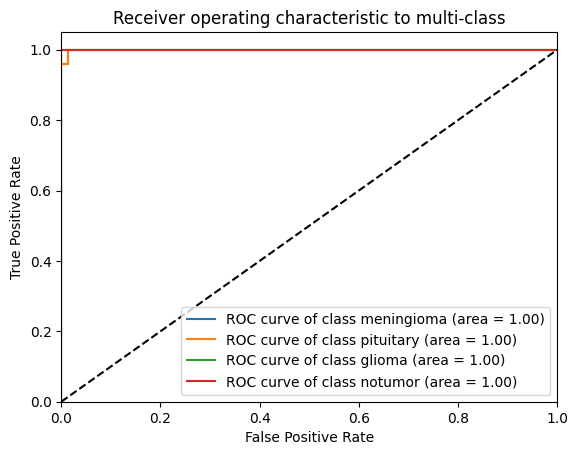
\includegraphics[width=\textwidth]{resnet50/evaluation/ROC.png}
    \caption{ROC Curve}
    \label{fig:resnet50_roc}
  \end{subfigure}
  \hfill
  \begin{subfigure}[b]{0.25\textwidth}
    \centering
    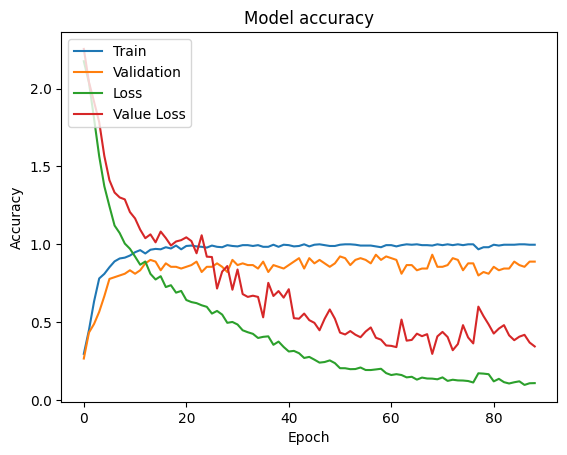
\includegraphics[width=\textwidth]{resnet50/evaluation/learning_curve.png}
    \caption{Learning Curve}
    \label{fig:resnet50_learning_curve}
  \end{subfigure}
  \caption{Confusion Matrix, Normalized Confusion Matrix, ROC Curve, and Learning Curve for Brain Tumor Segmentation}
  \label{fig:resnet50_evaluation}
\end{figure}

\begin{table}[ht]
\centering
\begin{tabular}{cc}
    \begin{minipage}{.6\linewidth}
        \centering
        \begin{subtable}[t]{\linewidth}
            \centering
            \begin{tabular}{|l|c|c|c|c|}
                \hline 
                \textbf{Class} & \textbf{Precision} & \textbf{Recall} & \textbf{F1-Score} & \textbf{Support} \\ 
                \hline 
                glioma      & 0.88 & 0.88 & 0.88 & 24 \\ 
                \hline
                meningioma  & 0.83 & 0.79 & 0.81 & 24 \\ 
                \hline
                notumor     & 0.89 & 1.00 & 0.94 & 24 \\ 
                \hline
                pituitary   & 1.00 & 0.92 & 0.96 & 24 \\ 
                \hline
                micro avg   & 0.90 & 0.90 & 0.90 & 96 \\ 
                \hline
                macro avg   & 0.90 & 0.90 & 0.90 & 96 \\ 
                \hline
                weighted avg & 0.90 & 0.90 & 0.90 & 96 \\ 
                \hline
                samples avg & 0.90 & 0.90 & 0.90 & 96 \\ 
                \hline
            \end{tabular}
            \caption{Classification Report for Brain Tumor Segmentation} 
            \label{tab:resnet50_classification_report}
        \end{subtable}
    \end{minipage} &
    \begin{minipage}{.35\linewidth}
        \centering
        \begin{subtable}[t]{\linewidth}
            \centering
            \begin{tabular}{|c|c|}
                \hline 
                \textbf{Metric} & \textbf{Value} \\ 
                \hline
                DSC & 0.8953 \\ 
                \hline
                Sensitivity & 0.8958 \\ 
                \hline
                Specificity & 0.9652 \\ 
                \hline
                Accuracy & 0.8958 \\ 
                \hline
            \end{tabular}
            \caption{Additional Metrics for Brain Tumor Segmentation} 
            \label{tab:resnet50_additional_metrics}
        \end{subtable}
    \end{minipage}
\end{tabular}
\caption{Classification Report and Additional Metrics for Brain Tumor Segmentation using ResNet50}
\label{tab:combined_resnet50_metrics}
\end{table}

The confusion matrices in Figures \ref{fig:resnet50_cm1} and \ref{fig:resnet50_cm2}, provide a detailed view of the model's performance across the four brain tumor classes: meningioma, pituitary, glioma, and no tumor. The glioma and meningioma classes exhibit slightly lower but still commendable true positive rates of 0.88 & 0.79 respectively, indicating strong performance across all categories. The classification report in Table \ref{tab:resnet50_classification_report} summarizes the precision, recall, and F1-score for each class. The model demonstrates high precision and recall across all classes, with a notable F1-score of 0.96 for the pituitary class. The overall micro, macro, and weighted averages for precision, recall, and F1-score all stand at 0.90, reflecting consistent and reliable performance.

The ROC curve in Figure \ref{fig:resnet50_roc} displays the true positive rate against the false positive rate for each class. The areas under the curve (AUC) for pituitary and no tumor classes are both perfect at 1.00, while meningioma and glioma classes show AUCs of 0.96 and 0.99, respectively, indicating excellent discriminative ability of the model.

The learning curve in Figure \ref{fig:resnet50_learning_curve} illustrates the model's accuracy and loss over 50 epochs. The plot shows the progression of training and validation accuracy, as well as loss and validation loss. The training accuracy remains relatively stable, while the validation accuracy also shows a stable trend, indicating effective learning. The training loss decreases gradually, and the validation loss fluctuates but generally maintains a downward trend. These trends suggest that the model is learning effectively without significant overfitting, as the validation metrics align closely with the training metrics. However, some oscillations in the validation loss curve may indicate areas for further optimization and can be attributed to the relatively small size of the dataset used. The limited data can lead to variability in how the model generalizes from one validation batch to another, resulting in the observed fluctuations.

Table \ref{tab:resnet50_additional_metrics} highlights the Dice Similarity Coefficient (DSC), sensitivity, specificity, and accuracy of the model. The DSC of 0.8953 indicates a good overlap between the predicted and actual tumor regions, reflecting the model's proficiency in segmentation tasks. The sensitivity and accuracy, both at 0.8958, demonstrate the model's capability to correctly identify true positives with a high degree of precision. Additionally, the specificity of 0.9652 highlights the model's effectiveness in accurately identifying true negatives, ensuring reliable performance in distinguishing between different classes of brain tumors.

\subsubsection{K-Folds Cross-Validation}

\begin{figure}[H]
  \centering
  \begin{subfigure}[b]{0.45\textwidth}
    \centering
    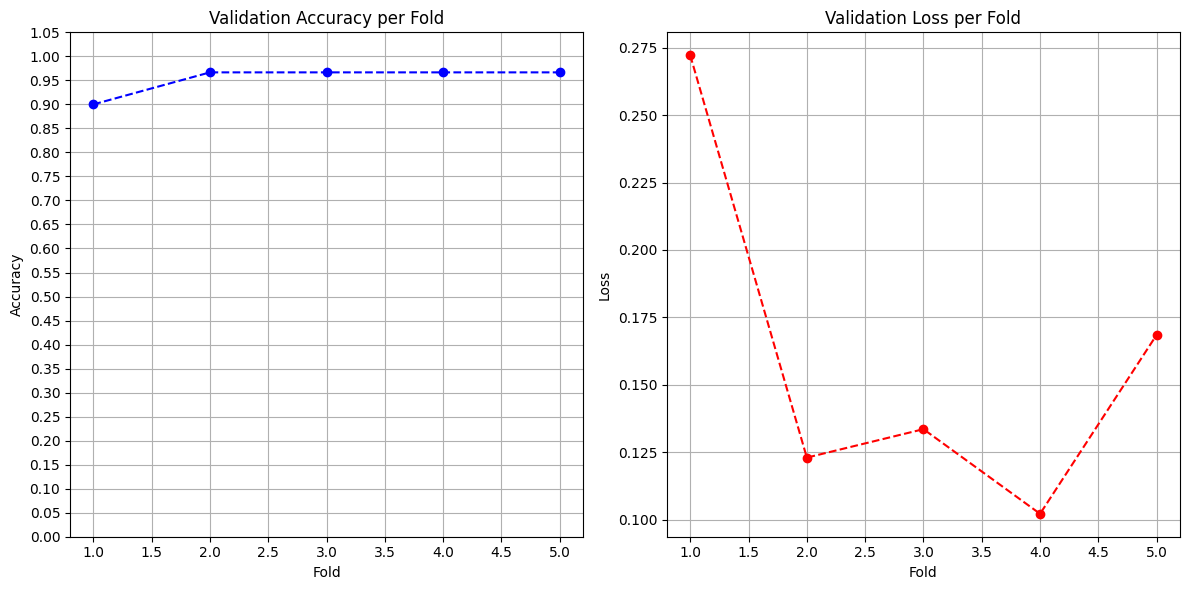
\includegraphics[width=\textwidth]{resnet50/evaluation/kfolds.png}
    \caption{Stratified K-Folds Cross-Validation for Brain Tumor Segmentation}\label{f:resnet50_kfolds}
  \end{subfigure}
  \hfill
  \begin{subfigure}[b]{0.45\textwidth}
    \centering
    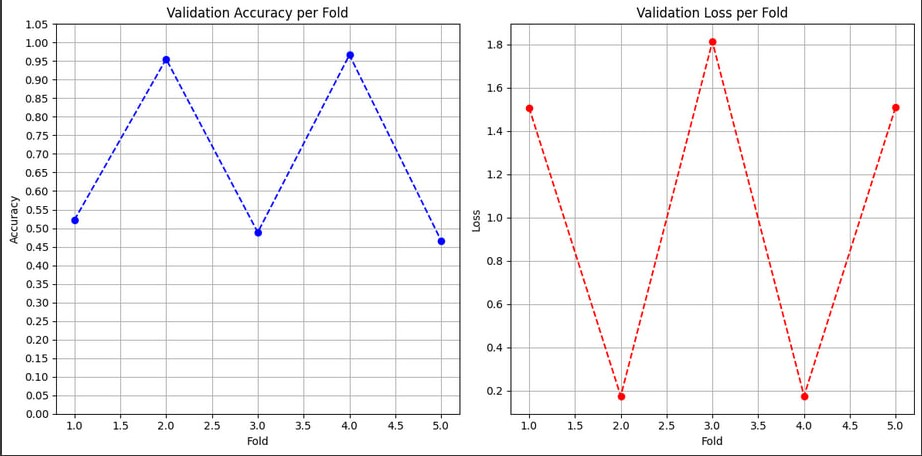
\includegraphics[width=\textwidth]{resnet50/evaluation/kfolds_5.jpg}
    \caption{K-Folds Cross-Validation for Brain Tumor Segmentation}\label{f:resnet50_kfolds_5}
  \end{subfigure}
  \caption{Comparison of Stratified K-Folds and K-Folds Cross-Validation for Brain Tumor Segmentation}\label{f:resnet50_kfolds_comparison}
\end{figure}

Stratified K-Folds cross-validation was meticulously conducted to evaluate the generalization performance of the ResNet50 model on the brain tumor classification task. The dataset was divided into ten folds, with each fold serving as a validation set once, while the remaining nine folds were used for training. This approach ensures that each class is well represented in both the training and validation sets across all folds, providing a robust estimate of the model's performance on unseen data. The model was trained for up to 80 epochs for each fold, with early stopping applied to halt training if the validation loss did not improve, thus preventing overfitting.

The left plot in Figure \ref{f:resnet50_kfolds} illustrates the validation accuracy for each fold. show significant variability in model performance across the ten folds. The validation accuracy achieved a mean of 0.8675 with a standard deviation of 0.1789, reflecting strong but variable performance. This variation in accuracy values, which ranged from approximately 0.50 to 1.00, highlights that while the model generally achieves high performance, there are instances where it performs less consistently, likely due to the specific characteristics of the validation set.

The right plot in Figure \ref{f:resnet50_kfolds} presents the validation loss for each fold. The validation loss averaged at 0.4642 with a standard deviation of 0.5849, as shown in the right plot. This significant variability in loss values suggests that while the model performs well overall, there are some folds where the performance is notably poorer. The large spikes in loss for some folds indicate areas where the model struggles to generalize, underscoring the need for further optimization to achieve more consistent results across different data subsets.

It is noteworthy that during some folds of the Stratified K-Folds cross-validation, the validation loss was lower than the training loss, and the validation accuracy was higher. This suggests that the model is robust and generalizes well to unseen data. However, this counterintuitive phenomenon can be attributed to the balanced distribution of classes in each fold, which is characteristic of stratification. While stratified sampling ensures each validation set is representative of the overall dataset, differences in data distribution between the training and validation sets can still occur, leading to higher accuracy and lower loss on the validation set for some folds. This might result in slightly overestimated performance metrics. Therefore, it is crucial to interpret these results with caution and consider the variability across all folds for a realistic assessment of the model's performance.

The comparison between the number of folds using normal K-Folds and Stratified K-Folds cross-validation, as illustrated in Figure \ref{f:resnet50_kfolds} and Figure \ref{f:resnet50_kfolds_5} demonstrates clear benefits of stratification. The normal K-Folds cross-validation shows significant variability in validation accuracy and loss across folds, suggesting inconsistent model performance. In contrast, the Stratified K-Folds results present a more stable and balanced performance, reflecting a more accurate representation of the model's capabilities.

Overall, the Stratified K-Folds cross-validation results demonstrate that the model achieved an average validation accuracy of 0.8675 with a standard deviation of 0.1789, indicating robust performance with some variability across folds. The average validation loss of 0.4642, with a standard deviation of 0.5849, suggests that while the model's predictions are generally reliable, there is room for improvement in reducing prediction errors. These metrics collectively indicate that the model has strong generalization capabilities, though further refinements could enhance the consistency and reliability of its performance across diverse data subsets. The results reinforce the value of Stratified K-Folds cross-validation in producing more reliable performance metrics, providing a clearer insight into the model's true potential on complex and varied datasets.

\subsubsection{Conclusion}\label{s:conclusion}

In this study, we developed and fine-tuned the ResNet50 model to address the challenging task of brain tumor classification. ResNet50's architecture, which utilizes residual connections to prevent vanishing gradients, was pivotal in building a robust and deep neural network capable of high performance. By leveraging these connections, we were able to train the model effectively across multiple layers, leading to accurate and reliable predictions for brain tumor classification. The model was specifically tailored to this task by excluding the top layers of the pre-trained ResNet50 and integrating layers that align with our classification objectives.

We employed a methodical approach to fine-tune the model, utilizing the Optuna framework to optimize hyperparameters, particularly focusing on the dropout rate to mitigate overfitting. The optimal dropout rate was determined through multiple trials, ensuring the model achieved the lowest possible validation loss while maintaining robust performance. This fine-tuning process demonstrated the importance of careful hyperparameter selection in enhancing the model's accuracy and reliability. The final model was configured with a dropout rate that balanced model complexity and performance, resulting in effective classification of brain tumor images.

To evaluate the model's performance, we implemented Stratified K-Folds cross-validation, which ensured each class was equally represented in each fold. This approach was crucial in providing a more accurate measure of the model's performance on unseen data, particularly in the context of a potentially imbalanced dataset. The results from this cross-validation method highlighted the model's ability to generalize well, achieving an average validation accuracy of 0.8675 and a validation loss of 0.4642 across ten folds. These metrics indicate the model's robustness and reliability in handling diverse data subsets.

The comparative analysis between normal K-Folds and Stratified K-Folds cross-validation underscored the advantages of stratification. Stratified K-Folds provided a more consistent and balanced evaluation of the model's performance, reducing the variability in accuracy and loss across folds observed in normal K-Folds cross-validation. This consistency underscores the importance of stratification in achieving more reliable performance metrics, particularly for datasets with imbalanced classes, and highlights the robustness of the ResNet50 model in various validation scenarios.

Overall, the study demonstrates the effectiveness of the ResNet50 model, combined with advanced optimization techniques and stratified cross-validation, in achieving accurate and reliable brain tumor classification. The high precision and recall achieved across different tumor classes indicate the model's potential for clinical applications. With further refinements and potential enhancements, such as improved data augmentation techniques or increasing the dataset used for training and evaluation, the model's performance can be further elevated, making it a valuable tool for brain tumor diagnosis and treatment planning. This work sets the stage for future research aimed at enhancing deep learning models for complex medical imaging tasks.
